\documentclass[11pt,a4paper]{ctexart}
\usepackage[margin=2.35cm]{geometry}
\usepackage{amsmath,amssymb}
\usepackage{tikz}
\usetikzlibrary{arrows.meta,positioning}
\usepackage{hyperref}
\usepackage{enumitem}
\usepackage{caption}
\usepackage{float}
\hypersetup{colorlinks=true,linkcolor=black,urlcolor=blue!55!black,pdftitle={DES 领域总览},pdfauthor={秋木}}
\setlength{\parindent}{2em}
\setlength{\parskip}{0.35em}
\setlist[itemize]{topsep=0.3em,itemsep=0.1em}
\captionsetup{font=small,labelformat=empty,justification=raggedright,singlelinecheck=false}
\tikzset{state/.style={circle,draw,minimum size=9mm,inner sep=0pt},arr/.style={-{Stealth[length=2.3mm]},thin}}

\title{DES 领域总览}
\author{秋木}
\date{2026 年 10 月 30 日}

\begin{document}
\maketitle

在阅读本篇博客之前，我希望读者对\textbf{有限状态自动机}(FSA, i.e. Finite State Automata)以及\textbf{带标签的有限状态自动机}(LFSA, i.e. Labeled Finite State Automata)有基本的了解。如果读者尚未接触过这个概念，可移步: [新建文件夹，博客正在装修中...]

言归正传，首先介绍一下在 DES 领域中常用的几个数学框架:
\begin{itemize}
  \item supervisory control theory on finite state automata;
  \item Petri net;
  \item Queueing System;
  \item Max-plus System;
\end{itemize}

以及领域中主要的两类性质:
\begin{itemize}
  \item inference-based properties;
  \item concealment-based properties;
\end{itemize}

在过去接近 40 年的研究中，围绕这些性质所提出的算法都依赖于两个基本假设：\textbf{deadlock freeness}(also, always run) and \textbf{divergence freeness}. 我们稍后会给出这两个性质的详细定义，不过粗略地说，第一个性质表示自动机可以一直运行，而第二个性质表示自动机没有可达的不可观测环。下面给出和这两个性质相关的几个例子，来帮助读者更好地理解它们。

\begin{figure}[H]
\centering
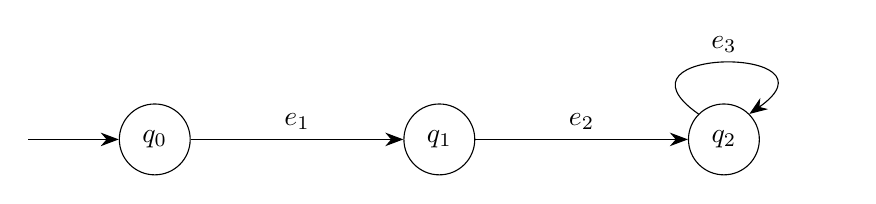
\begin{tikzpicture}[node distance=2.7cm]
  \node[state] (q0) {$q_0$}; \node[state,right=of q0] (q1) {$q_1$}; \node[state,right=of q1] (q2) {$q_2$};
  \draw[arr] ([xshift=-1.15cm]q0.west) -- (q0.west);
  \draw[arr] (q0) -- node[above] {$e_1$} (q1);
  \draw[arr] (q1) -- node[above] {$e_2$} (q2);
  \draw[arr] (q2.north west) to[out=145,in=35,looseness=6] node[above] {$e_3$} (q2.north east);
\end{tikzpicture}
\caption{图 1：$q_2$ 可以通过 $e_3$ 不断转移；所以这个自动机是 deadlock free 的。}
\end{figure}

\begin{figure}[H]
\centering
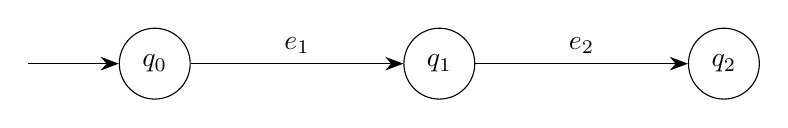
\begin{tikzpicture}[node distance=2.7cm]
  \node[state] (q0) {$q_0$}; \node[state,right=of q0] (q1) {$q_1$}; \node[state,right=of q1] (q2) {$q_2$};
  \draw[arr] ([xshift=-1.15cm]q0.west) -- (q0.west);
  \draw[arr] (q0) -- node[above] {$e_1$} (q1);
  \draw[arr] (q1) -- node[above] {$e_2$} (q2);
\end{tikzpicture}
\caption{图 2：移除 $e_3$ 后，$q_2$ 成为死锁状态; 所以这个自动机不是 deadlock free 的。}
\end{figure}

\begin{figure}[H]
\centering
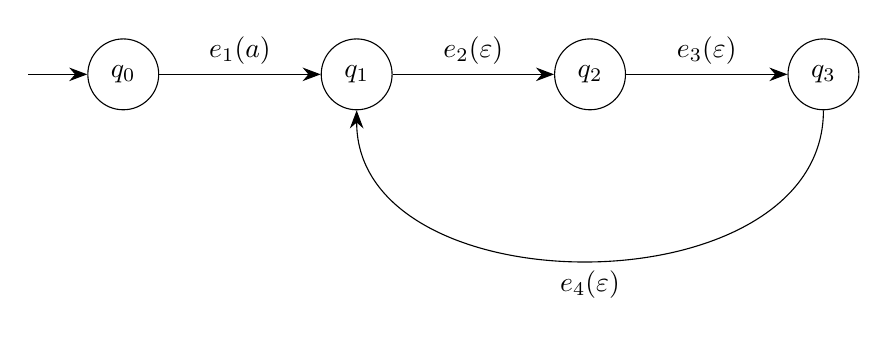
\begin{tikzpicture}[node distance=2.05cm]
  \node[state] (q0) {$q_0$}; \node[state,right=of q0] (q1) {$q_1$}; \node[state,right=of q1] (q2) {$q_2$}; \node[state,right=of q2] (q3) {$q_3$};
  \draw[arr] ([xshift=-0.75cm]q0.west) -- (q0.west);
  \draw[arr] (q0) -- node[above] {$e_1(a)$} (q1);
  \draw[arr] (q1) -- node[above] {$e_2(\varepsilon)$} (q2);
  \draw[arr] (q2) -- node[above] {$e_3(\varepsilon)$} (q3);
  \draw[arr] (q3.south) to[out=-90,in=-90,looseness=1.1] node[below] {$e_4(\varepsilon)$} (q1.south);
\end{tikzpicture}
\caption{图 3：$q_1\to q_2\to q_3\to q_1$ 构成不可观测环；所以这个自动机不是 divergence free 的。}
\end{figure}

\begin{figure}[H]
\centering
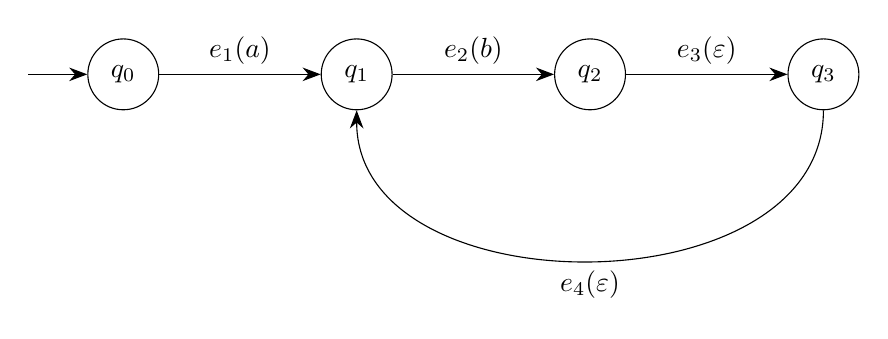
\begin{tikzpicture}[node distance=2.05cm]
  \node[state] (q0) {$q_0$}; \node[state,right=of q0] (q1) {$q_1$}; \node[state,right=of q1] (q2) {$q_2$}; \node[state,right=of q2] (q3) {$q_3$};
  \draw[arr] ([xshift=-0.75cm]q0.west) -- (q0.west);
  \draw[arr] (q0) -- node[above] {$e_1(a)$} (q1);
  \draw[arr] (q1) -- node[above] {$e_2(b)$} (q2);
  \draw[arr] (q2) -- node[above] {$e_3(\varepsilon)$} (q3);
  \draw[arr] (q3.south) to[out=-90,in=-90,looseness=1.1] node[below] {$e_4(\varepsilon)$} (q1.south);
\end{tikzpicture}
\caption{图 4：不含有不可观测环，因此是 divergence free 的。}
\end{figure}

如果暂时不理解这些例子也没关系，之后我给出这两个性质的严格定义之后，读者可返回检查这些例子。

\bigskip\hrule\bigskip

接下来，我来介绍一下 $\omega$-strong detectability（$\omega$-强可检测性），这是一个 inference-based property, 即根据观测推测系统当前状态。

\textbf{定义}（参见 \href{https://doi.org/10.1007/s10626-018-0268-y}{Sasi \& Lin, 2018, Definition 1}；以下采用 \href{https://doi.org/10.1016/j.arcontrol.2023.100902}{Zhang, 2023} 的 LFSA 记号）：一个带标签的有限状态自动机 $\mathcal{S}$ 是 $\omega$-强可检测的，当且仅当存在正整数 $k$，使得对每条无限事件轨迹 $s\in L^\omega(\mathcal{S})$，以及 $\ell(s)$ 的每个满足 $|\sigma|>k$ 的前缀 $\sigma$，都有
\[
  |\mathcal{M}(\mathcal{S},\sigma)|=1.
\]

这里，$\ell(s)$ 是轨迹 $s$ 产生的观测序列；$\mathcal{M}(\mathcal{S},\sigma)$ 是观察到 $\sigma$ 后所有可能的当前状态组成的集合。也就是说，经过统一的观测长度阈值 $k$ 后，任意无限轨迹上的当前状态都能被唯一确定。

这里存在一个很常见的误解：看上去，最终的结果好像只和 $\sigma$ 的长度有关，而 $s$ 出现在定义叙述中的意义看起来并不显然。一个重要的事实是，在 $\mathcal{L}(G)$ 中所有长度超过为 $k$ 的标签序列的集合，与本题定义中所取出的所有长度超过 $k$ 的标签序列的集合并不相等。我们可以把这两个集合写出，然后用一个例子来说明它们为什么不等价。给定 $k$:
\[
S_1 := \{\sigma\in\mathcal{L}(G)\mid \exists s\in L^\omega(G),\ \sigma\sqsubset\ell(s),\ |\sigma|>k\},
\]
\[
S_2 := \{\sigma\in\mathcal{L}(G)\mid |\sigma|>k\}.
\]

其中 $\sigma\sqsubset\ell(s)$ 表示 $\sigma$ 是无限观测序列 $\ell(s)$ 的前缀。

$S_1$ 定义中的特殊之处在于，$s$ 的存在限定了标签序列 $\sigma$ 至少可以产生于一个能导向环的 event 路径。而对于任意一个足够长的标签序列，其未必能由这样的 event 序列得到。下面给出一个例子，来更好地展现这两个集合之间的差异：

\begin{figure}[H]
\centering
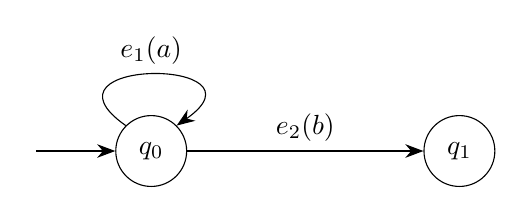
\begin{tikzpicture}[node distance=3.0cm]
  \node[state] (q0) {$q_0$}; \node[state,right=of q0] (q1) {$q_1$};
  \draw[arr] ([xshift=-1.0cm]q0.west) -- (q0.west);
  \draw[arr] (q0) -- node[above] {$e_2(b)$} (q1);
  \draw[arr] (q0.north west) to[out=145,in=35,looseness=6] node[above] {$e_1(a)$} (q0.north east);
\end{tikzpicture}
\end{figure}

对于这个例子，
\[
L^\omega(G)=\{e_1^\omega\},\qquad S_1=\{a^n\mid n>k\},
\]
而所有足够长、可由系统产生的有限标签序列组成
\[
S_2=\{a^n\mid n>k\}\cup\{a^n b\mid n\ge k\}.
\]

\section*{预告}

后面我们会给出曾经的论文中用于验证这个性质的算法。这个算法开始要求系统满足两个基本性质，但是在后来的推广中去掉了这两个性质。但是，Zhang 在 2023 年发表的论文称这个新算法在移除了两个基本假设之后是错误的，并给出了反例。在之后的博客中，我们会逐一验证这些说法，然后介绍 Zhang 提出的新方法。

之后，我们还会介绍其他基本性质：
\begin{itemize}
  \item diagnosability;
  \item predictability;
  \item opacity;
\end{itemize}

\end{document}
